\documentclass[a4paper,fleqn,11pt]{article}

%\usepackage{times}
\usepackage{natbib}
\usepackage{rotating}
\usepackage{longtable, lscape}
\usepackage{threeparttablex}
\usepackage{amsmath}
\usepackage{amssymb}
\usepackage{latexsym}
%\usepackage[top=2.5cm, bottom=2.5cm, left=2cm , right=1.8cm]{geometry}
\usepackage[pdftex,svgnames]{xcolor}
\usepackage{verbatim}
\usepackage{pictexwd}
%\usepackage{supertabular}
%\usepackage{tabls}
%\usepackage{url}

\usepackage{enumitem}

\usepackage[pdfstartview={},
            pdftex,
%            pdftitle=RSiena\ Manual,
            pdfdisplaydoctitle,
            plainpages=false,
            bookmarks=true,
            bookmarksopen=true,
            bookmarksnumbered=true,
            colorlinks,
            linkcolor=Crimson,
            anchorcolor=Maroon,
            citecolor=MidnightBlue,
            urlcolor=VioletRed
            ]{hyperref}

\setlength{\bibsep}{0.01in}

%\setlength{\oddsidemargin}{15mm}


%\usepackage[pdftex]{graphicx}
%\usepackage[pdftex,dvipsnames]{color}

%%\renewcommand\floatpagefraction{1}
%\renewcommand\textfraction{0}

%\def\bibsection{\section{\refname}}
\renewcommand\bibsection{\section{\refname}}

\newcommand{\opmerking}[1]{\par \fbox{\Large #1} \par}
%\newcommand{\opmerking}[1]{}
\newcommand{\ch}{\mbox{$\chi^{2}$ }}
\newcommand{\boldpi}{\mbox{\boldmath$\pi$ }}
\renewcommand{\l}{\mbox{$\lambda$ }}
\newcommand{\informationy}{\mbox{${\cal E}$}}
\newcommand{\var}{\mbox{var}}
\newcommand{\cov}{\mbox{cov}}
\newcommand{\mathbold}[1]{\mbox{\boldmath $\bf#1$}}
\newcommand{\Reals}{\mbox{I} \! \mbox{R}}
\newcommand{\+}{\, + \,}
\renewcommand{\min}{\, - \,}
\newcommand{\half}{{\textstyle \frac{1}{2}}}
\newcommand{\neqsum}[3]
{\, \sum_{\stackrel{\scriptstyle #1 = 1}{\scriptstyle #2 \neq #3}}^n \,}
\newcommand{\vit}{\theenumi}

\newcommand{\firsttabitem}{\hspace{4mm} $\bullet$ \hspace{1mm}}
\newcommand{\tabitem}{\\ \\ \hspace{4mm} $\bullet$ \hspace{1mm}}

\newcommand{\E}{\mbox{$\cal E$}}
\renewcommand{\P}{\mbox{P}}
\newcommand{\se}{\mbox{s.e.}}

\newcommand{\sfn}[1]{\textsf{#1}}

\newcommand{\R}{{\sf R }}
\newcommand{\Rn}{{\sf R}}
\newcommand{\rs}{{\sf RSiena}}
\newcommand{\RS}{{\sf RSiena }}
\newcommand{\SI}{{\sf SIENA }}
\newcommand{\SN}{{\sf StOCNET }}
\newcommand{\si}{{\sf SIENA}}
\newcommand{\sn}{{\sf StOCNET}}

\newcommand{\mcc}[2]{\multicolumn{#1}{c}{#2}}
\newcommand{\mcp}[2]{\multicolumn{#1}{c|}{#2}}

\renewcommand{\th}[1]{$\theta_{#1}$}
\newcommand{\be}[1]{$\beta_{#1}$}
\newcommand{\ga}[1]{$\gamma_{#1}$}
\newcommand{\beq}{\begin{equation}}
\newcommand{\eeq}{\end{equation}}
%\renewcommand{\bibitem}[1]{\bigskip \par \noindent \hspace{-4pt}}
\makeatletter
\newenvironment{indentation}[2]
{\par \setlength{\leftmargin}{#1}       \setlength{\rightmargin}{#2}
  \advance\linewidth -\leftmargin       \advance\linewidth -\rightmargin
  \advance\@totalleftmargin\leftmargin  \@setpar{{\@@par}}%
  \parshape 1 \@totalleftmargin         \linewidth \ignorespaces}{\par}
\makeatother
%\renewcommand{\bibitem}[1]{\par \noindent \hskip-\parindent}

\newcommand{\separationb}{\\[0.5ex]\hline\rule{0pt}{2ex}}


\newcounter{savenumi}

\newenvironment{startenum}
{\begin{enumerate}}{\setcounter{savenumi}{\value{enumi}\end{enumerate}}}

\newenvironment{followenum}
{\begin{enumerate}\setcounter{enumi}{\value{savenumi}}}
{\setcounter{savenumi}{\value{enumi}\end{enumerate}}}

\newcounter{thisno}
\newcommand{\startno}{\setcounter{thisno}{0}}
\newcommand{\nextno}{\addtocounter{thisno}{1}\thethisno .\ }

\hyphenation{Snij-ders Duijn Huis-man Steg-lich Schwein-ber-ger siena-Data-Create-From-Session}

\newcommand{\interruptenum}{
      \setcounter{savenumi}{\value{enumi}}
      \end{numlijst}
      \end{slid} \begin{slid}
      \begin{numlijst}
      \setcounter{lijstnum}{\value{savenumi}}}

%\renewcommand{\baselinestretch}{1.2}


\setlength{\oddsidemargin}{0.6cm}
\setlength{\textwidth}{15cm}

\ifx\pdfoutput\undefined
\else
  \ifx\pdfoutput\relax
  \else
    \ifnum\pdfoutput>0
      % PDF output
      \pdfminorversion=5
      \pdfcompresslevel=9
      \pdfobjcompresslevel=3
    \fi
  \fi
\fi

\title{{\Huge Using the siena01Gui for \textsf{RSiena} } }
%\protect\newline \normalsize } }
\author{\Large Ruth M.\ Ripley\\[1ex]
        \Large Tom A.B.\ Snijders\\[1ex]
       {\large University of Oxford: Department of Statistics; Nuffield College}\\[1ex]
    }
%\date{}

\definecolor{lc}{cmyk}{0,0.5,0,0.5}

\begin{document}

\maketitle

%\setlength{\unitlength}{1mm}
%\begin{picture}(100,100)
%\put(0,0){\includegraphics*[scale=4]{ilcampo.jpg}}
%\end{picture}
\vfill
\begin{center}
\includegraphics*[scale=3]{ilcampo.jpg}
\end{center}
\vfill
%\addtocontents{toc}{\setlength{\parsep}{1pt plus1pt minus1pt}}

%\addtocontents{toc}{\setlength{\itemsep}{1pt plus1pt minus1pt}}

\makeatletter
\def\@linkcolor{lc}
\makeatother



\section{How to start \SI using the \sfn{siena01Gui}}
\label{S_minsi1}

Next to data input in the normal way for  \Rn, described in the manual
and the help pages, data input for \SI can also be done
using the  graphical user interface (\emph{GUI}) via \textsf{siena01Gui()}.
The latter way is not favored by the \SI maintainers,
but it still is available and documented here in
a minimal cookbook-style introduction.


\subsection{Data formats}
\label{S_datform}

\begin{enumerate}
\item
Network and covariate files should be text files with a row for each node. The
numbers should be separated by spaces or tabs.
\item
An exogenous events file can be given, indicating change of composition of the
network in the sense that some actors are not part of the network during
all the observations.
This will trigger treatment of such change of composition
according to \citet{HuismanSnijders03}.
This file must have one row for each node.
Each row should be
consist of a set of pairs of numbers which indicate the periods
during which the corresponding actor
was present. For example,
\begin{verbatim}
1 3
1.5 3
1 1.4 2.3 3
2.4 3
\end{verbatim}
would describe a network with 4 nodes, and 3 observations. Actor 1 is present
all the time, actor 2 joins at time 1.5, actor 3 leaves and time 1.4 then
rejoins at time 2.3, actor 4 joins at time 2.4. All intervals are treated as
closed.
\item If you use software such as Excel or SPSS to create input files to use
  with \RS on a Mac, try to ensure that you do not create Unicode\footnote{Unicode
  is one of the standards for encoding text, an alternative to ASCII.
  Unicode formats are denoted by symbols such as UTF-8 and UCS-2.} files. This
  is an option in SPSS, and will depend on the file type with Excel.
\end{enumerate}

More about input data can be found in the manual.

\subsection{Installation and running the graphical user interface under Windows}
\label{Gui}
\begin{enumerate}
\item % Install the \RS version of \Rn.
  Install \R (most recent version). Note that if this leads to any
  problems or questions, \R has an extensive list of `frequently asked
  questions' which may contain adequate help for you.\\
  Start \Rn, click on \sfn{Packages} and
  then on \sfn{Install packages(s)...}. You will be prompted to select a mirror
  for download. Then select the packages \sfn{xtable},
  \sfn{network}
  and \rs. \\
  If you are using some version of Windows and get an error of denied permission  when trying to install the packages,
  you may get around this by right-clicking the \R icon and selecting
  `Run as administrator'.
\item If you want to get the latest beta version of \rs, before installing the
  packages, select \sfn{Packages/Select repositories...} and select
  \sfn{R-forge}. Then install the packages in the normal way.
  (Sometimes the \SI website also contains newer versions.) \\
\item Start up \R from the start menu or by (double-)clicking a shortcut on
  the taskbar (or desktop).
\item By right-clicking the shortcut and clicking `Properties'
      you can change the startup working directory, given in the
      `Start in' field. Data files will be searched for in the first instance
      in this directory.
\item Load the \RS package via the menu \texttt{Packages}
\item Type\\
\verb|siena01Gui()|
\item You should see a screen like that shown in \hyperlink{siena1}{Figure
    \ref{fig:siena1}}
  \begin{figure}[ht]
    \begin{center}
      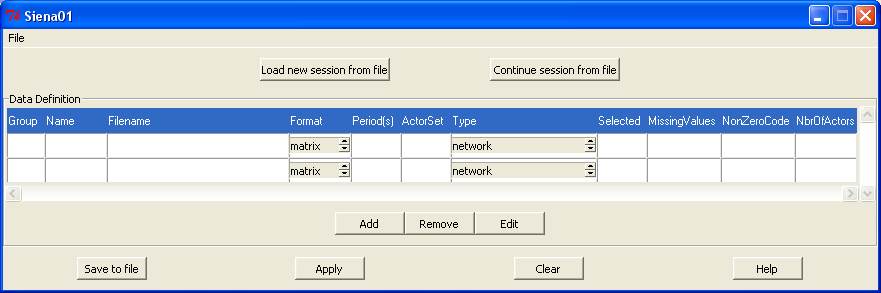
\includegraphics[width=\textwidth]{siena1.png}
\hypertarget{siena1}{}
    \end{center}
\caption{Siena Data Entry Screen}
\label{fig:siena1}
  \end{figure}
\item If the initial screen appears correctly, then check your working directory
  or folder. This is the directory that is opened immediately when clicking the
  \textsf{Add} button.  Various problems can be avoided by making sure that the
  working directory is the directory that also contains the data files and the
  saved session file
  (see below)!\\
  You need to have permission to write files in the working directory, and the
  data files you want to use need to be in the same directory. To change the
  directory:
\begin{enumerate}
\item Right click on the shortcut, and select Properties. (if somehow you don't
  have permission to do this, try copying the shortcut and pasting to create
  another with fewer restrictions. (This may not work in Windows 7: you may need
  to copy it from the visible desktop and then paste it in Windows Explorer in
  your personal Desktop area.))  In the \textsf{Start in:} field type the name
  of the directory in which you wish to work, i.e., a directory in which you can
  both read and write files. Then click OK.

\item To run the examples, put the session file and the data files in
the chosen directory before starting \rs.

\item To use your own data, put that data in the chosen directory before
starting \rs.
\end{enumerate}
\end{enumerate}

\subsubsection{Using the graphical user interface from Mac or Linux}
\begin{enumerate}
\item Install \R (most recent version) as appropriate for your computer.
\item Within \Rn, type\\
  \sfn{install.packages("RSiena")}\\
To use the latest beta version, use\\
 \sfn{install.packages("RSiena", repos="http://R-Forge.R-project.org")}

%  \sfn{install.packages("RSiena", repos="http://www.stats.ox.ac.uk/pub/RWin")}

%\item It is possible that Mac users on `Tiger' will need\\
%  \sfn{install.packages("RSiena", repos="http://www.stats.ox.ac.uk/pub/RWin",
%    type="source")}
\item Navigate to the directory RSiena package, (which you can find from within
  R by running \sfn{system.file(package="RSiena")}) and find a file called
  \sfn{sienascript}.  Run this to produce the Siena GUI screen.(You will
  probably have to change the permissions first (e.g.\ \\ \textsf{chmod u+x
    sienascript})).
\item If you want to use the GUI, you need tcl/tk installed. This is an
  (optional) part of the R installation on Mac. On Linux, you may need to
  install Tcl/tk and the extra Tcl/tk package \sfn{tktable}. On
  Ubuntu Linux, the following commands will do what is
  necessary (perhaps version numbers must be adapted):\protect\footnote{Thanks
  to Michael Schweinberger and Krists Boitmanis for supplying these commands.}
\begin{verbatim}
sudo apt-get install tk8.5
sudo apt-get install libtktable2.9
\end{verbatim}
\end{enumerate}

\subsubsection{Running  the graphical user interface: more details}
\label{S_guiinR}

Originally \RS provided access to the GUI interface direct from Windows. This is
not now possible. This section details some helpful notes about starting \RS
within R\protect\footnote{We are
grateful to Paul Johnson for supplying
these ideas.}.
This is done by starting up \R and working with the following commands.
Note that \R is case-sensitive, so you must use upper and lower
case letters as indicated.

First, set the `working directory' of the \R session
to the same directory that holds the data files;
for example,\\
\sfn{setwd('C:/SienaTest')}

\noindent (Note the forward slash\protect\footnote{You can use backward ones but they
 must be doubled: \sfn{setwd('C:\textbackslash\textbackslash SienaTest')}.},
 and the quotes are necessary\protect{\footnote{Single or double, as long as they match.}.)
Windows users can use the \sfn{Change dir...} option on the \sfn{File} menu.

You can use the following commands to make sure the working directory is
what you intend and see which files are included in it:\\
\sfn{ getwd()}\\
\sfn{ list.files()}

Assuming you see the data files, then you can proceed to load the
\RS package, with the library function:\\
\sfn{ library(RSiena)}\\
The other packages will be loaded as required, but if you wish to examine them
or use other facilities from them you can load them using:\\
\sfn{ library(network)}\\
The following command
will give a review of
the functions that \RS offers:\\
\sfn{ library(help=RSiena)}\\
After that, you can use the \RS GUI. It will `launch' out
of the \R session.\\
\sfn{ siena01Gui()}\\
You can monitor the \R window for error messages -- sometimes they are
informative.

When you are done, quit \R in the polite way:\\
\sfn{q()} \\(Windows users may quit from the \sfn{File} menu or by closing the
window.)

\subsubsection{Entering Data.}
\label{thegui}
There are two ways to enter the data.
\begin{enumerate}
\item Enter each of your data files using \sfn{Add}.\\
      Fill in the various columns as described in Section~\ref{S_de_screen}.
\item If you have earlier saved the specification
      of data files, e.g., using \sfn{Save to file}, then you can
      use \sfn{Load new session from File}.\\
      This requires a file in the format described
      at the end of  Section~\ref{S_de_screen};
      such a file can be created and read in an editor or spreadsheet program,
      and it is created in .csv (comma separated) format
      by the \sfn{ siena01Gui()} when you request
      \sfn{Save to file}.
\item If you wish to remove files, use the \sfn{Remove} option rather than
  blanking out the entries.
\end{enumerate}
Once you have done this, check that the \sfn{Format},
\sfn{Period}, \sfn{Type}, etc., are correct, and enter any
values which indicate missingness in the \sfn{Missing Values} column.
A (minimal) complete screen is shown in \hyperlink{siena2}
{Figure~\ref{fig:siena2}}.
The details of this screen are explained in Section~\ref{S_de_screen}.
  \begin{figure}[ht]
\hypertarget{siena2}{}
    \begin{center}
      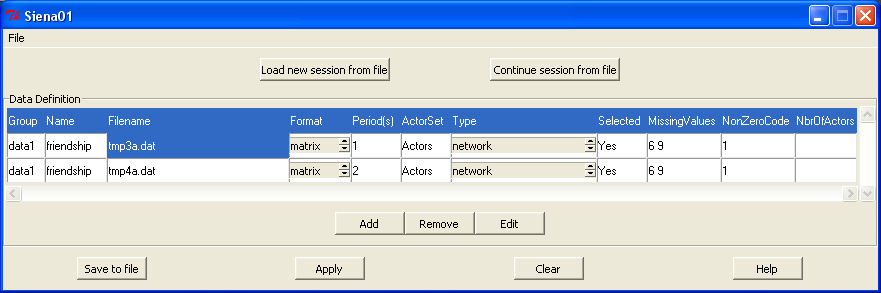
\includegraphics[width=\textwidth]{siena2.png}
    \end{center}
 \caption{Example of a Completed Data Entry Screen}
 \label{fig:siena2}
\end{figure}

\subsubsection{Running the Estimation Program}
\label{estgui}
\begin{enumerate}
\item Click \sfn{Apply}: you will be prompted to save your work. Then you should
  see the \sfn{Model Options} screen shown in \hyperlink{options}{Figure
    \ref{fig:options}}.
  \begin{figure}[ht]
      \hypertarget{options}{}
    \begin{center}
      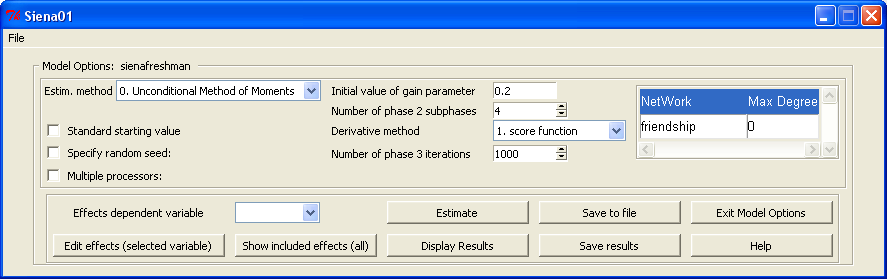
\includegraphics[width=\textwidth]{siena3.png}
    \end{center}
\caption{Model options screen}
\label{fig:options}
  \end{figure}
    If this does not happen, then one possible source of error is that the
    program cannot find your files; e.g.,
    the files are not in the working directory (see above) but in a different
    directory.\\
    If errors occur at this moment and the options screen does not appear,
    then you can obtain diagnostic error messages
    working not through the \sfn{siena01Gui}, but directly  within \R
    as described in Section~\ref{S_slightlyR}.
    This will hopefully help you solving this problem; later on
    you can then work through the \sfn{siena01Gui} again.
\item Select the options you require.
\item Use \sfn{Edit Effects} to choose the effects you wish to include. Note you
  can edit the effects for just one dependent variable at a time if you wish
  by selecting one dependent variable in `Effects dependent variable'.
\item Click \sfn{Estimate}.
\item You should see the \SI screen of the estimation program.
\item When the program has finished, you should see the results. If not, click
  \sfn{Display Results} to see the results.  The output file which you will see
  is stored, with extension \texttt{.out} in the directory in which you start
  \sfn{siena.exe}.
\item You may restart your estimation session at a later date using the
  \sfn{Continue session from file} on the \sfn{Data Entry Screen}.\\
  The restart needs a saved version of the data, effects and model as R
  objects. This will be created automatically when you first enter the
  \sfn{Model Options Screen}, using the default effects and model. You may save
  the current version at any time using the \sfn{Save to file} button, and will
  be prompted to do so when you leave this screen.
\end{enumerate}

\subsubsection{Details of The Data Entry Screen}
\label{S_de_screen}

\begin{description}
\item[\sfn{Group}] May be left blank unless you wish to use the
  \sfn{multi-group} option described in the manual. Should not
  contain embedded blanks.
\item[\sfn{Name}] Network files or dyadic covariates should use the same name
  for each file of the set. Other files should have unique names, a list of
  space separated ones for constant covariates.
\item[\sfn{File Name}] Usually entered by using a file selection box, after
  clicking \sfn{Add}.
\item[\sfn{Format}] Only relevant for networks or dyadic covariates. Can be
  a matrix; a single
  Pajek network (\sfn{.net}) (not for two-mode networks);
  or a \sfn{Siena network file} (an edgelist,
  containing three or four columns: (from, to, value, wave (optional)), not yet
  tested for dyadic covariates!).
  By specifying the waves in the fourth column in the \sfn{Siena} format,
  one file can be used to contain data for all the waves.
%(\sfn{.paj} file support will be added
  %later, with a specific button to load a complete project.)
\item[\sfn{Period(s)}] Only relevant for networks and dyadic covariates. All
  other files cover all the relevant periods. Indicates the order of the network
  and dyadic covariate files. Should range from 1 to \sfn{M} within each
  \sfn{group}, where \sfn{M} is the number of time points (waves).
  Use multiple numbers separated by spaces for multi-wave Siena
  network files.
\item[\sfn{ActorSet}] If you have more than one set of nodes, use this column to
  indicate which is relevant to each file. Should not contain embedded blanks.
\item[\sfn{Type}] Indicate here what type of data the file contains. Options
  are:
\begin{description}
\item[\sfn{network}] (i.e., a one-mode network, which is the
     usual type)
\item[\sfn{bipartite}] (i.e., a two-mode network, which is a network with two
    node sets, and all ties are between the first and the second node set)
\item[\sfn{behavior}]
\item[\sfn{constant covariate}]
\item[\sfn{changing covariate}]
\item[\sfn{constant dyadic covariate}]
\item[\sfn{changing dyadic covariate}]
\item[\sfn{exogenous event}] (for changing composition of the actor set)
\end{description}
\item[\sfn{Selected}] Yes or No. Files with \sfn{Yes} \emph{or blank} will be
included in the model. Use this field to remove any networks or behavior
variables that are not required in the model.
\item[\sfn{Missing Values}] Enter any values which indicate missingness, with
  spaces between different entries.
\item[\sfn{Nonzero Codes}] Enter any values which indicate ties, with spaces
  between different entries.
\item[\sfn{NbrOfActors}] For \sfn{Siena network files}, enter the number of
  actors. For \sfn{Siena net bipartite files}, enter the two dimensions
  (number of rows, number of columns) of the network, separated by a blank space.
 \end{description}

 The details of the screen can be saved to a \emph{session} file, from which
 they can be reloaded. But you can create a session file directly: it should
 have columns with exactly the same names and in exactly the same order as those
 of the \sfn{Data Entry} screen, and be of any of the following types:
\begin{center}
\begin{tabular}{lll}\\
Extension&Type\\
\texttt{.csv}&Comma separated\\
\texttt{.dat} or \texttt{.prn}&Space delimited\\
\texttt{.txt}&Tab delimited\\
\end{tabular}
\end{center}

\noindent
The root name of this input file will also be the root name of the output file.

\subsubsection{Continuing the estimation}
\begin{enumerate}
\item Below you will see some points about how to evaluate the reliability of
  the results.  If the convergence of the algorithm is not quite satisfactory
  but not extremely poor, then you can continue just by \textsf{Apply}ing the
  estimation algorithm again.
\item If the parameter estimates obtained are very poor (not in a reasonable
  range), then it usually is best to start again, with a simpler model, and from
  a standardized starting value.  The latter option must be selected in the
  \textsf{Model Options} screen.
\end{enumerate}

Section~\ref{S_guiToR} explains how to make the step from the use of the
GUI to the use of \R commands in the regular \R way.

\subsubsection{The transition from using the graphical user interface to commands}
\label{S_guiToR}

At some moment, for users who started learning the use of \RS through the GUI,
it can be desirable to make the transition to using commands in the regular \R way.
This will make available more options and integration with other \R features.
The transition can easily be made as follows.

After having made at least one estimation run
in the GUI (which could be with the default
model specification, without having made any further additions to the model;
but it could also be with a more complicated model), click the button
\sfn{Save to file}. You will be prompted for a file name with extension \sfn{.RData}.
Make sure that you do give a non-empty name before the dot in \sfn{.RData};
for the moment, let us choose the name  \sfn{trans.RData}.

Then later in an \R session you can load the  \sfn{trans.RData}.
This can be done in Windows by selecting \sfn{File -- Load Workspace} from the drop down
menu, and entering this file name. It can also be done by entering the command
\begin{verbatim}
load("trans.RData")
\end{verbatim}
This will make available three objects, for data, algorithm, and effects.
What is currently in your workspace is shown by the command
\begin{verbatim}
ls()
\end{verbatim}
This will probably show that the loaded objects have the names
\sfn{mydata}, \sfn{mymodel}, and \sfn{myeff}.
These are the type of objects created by the functions \sfn{sienaDataCreate},
\sfn{sienaAlgorithmCreate}, and \sfn{getEffects},
and discussed in the \SI script  \sfn{Rscript02SienaVariableFormat.R}
on the \SI website.

Now attach the package \RS and subsequently ask for the descriptions of these
three objects:
\begin{verbatim}
library(RSiena)
mydata
mymodel
myeff
\end{verbatim}
This will give short descriptions and thereby a confirmation of what has been
imported from the GUI session to the regular \R session.
From here on you can continue and work with \R commands,
as in the script, to further specify the model by working
on the effects object, and then estimate the parameters by the \sfn{siena07}
function.

The precise point to continue from here, using the scripts
in the next section and also on the \RS website,
is to use
script \sfn{Rscript02SienaVariableFormat.R},
starting with section~D (\emph{Defining Effects}),
part~3 (\emph{Adding/removing effects using includeEffects}).
After this, you are advised to continue with script
\sfn{Rscript03SienaRunModel.R}.

\end{document}
